\documentclass[12pt]{report}
\usepackage[T2A]{fontenc}
\usepackage[utf8]{inputenc}
\usepackage[english,russian]{babel}
\usepackage{amssymb,amsfonts,amsmath,mathtext, amsthm}
\usepackage{url, hyperref}
\usepackage{graphicx}
\usepackage{xfrac}

\newcommand{\sigSQUID}{\sigma_{SQUID}}
\newcommand{\Ab}{a_{\beta}}
\newcommand{\ntrl}{n}

\newtheorem{rmk}{Замечание}
\newtheorem{concl}{Вывод}

\title{Аргумент от точности определения среднего вертикального оффсета}

\begin{document}
	\maketitle
	
Целью данного теста является проверка возможности определения вертикального разделения замкнутых орбит пучков на уровне $10^{-12}$~м, если:
\begin{itemize}
	\item в ускорителе длины $L_{acc} = 150$~м равномерно распределены $N_{BPM}~=~25$ BPM;
	\item точность измерения вертикальной координаты пучка BPM'ом $\sigSQUID~=~10^{-12}$~м;
	\item амплитуда бетатронных колебаний в вертикальной плоскости $\Ab~=~10^{-6}$~м.
\end{itemize}

В нижеследующих тестах мы предполагали \emph{один} проход пучка через кольцо ускорителя ($N_{turn}=1$), так что на каждом триале мы имели по $N_{BPM}$ измерений положения пучка, на основании которых определялись вертикальные сдвиги замкнутых орбит пучков.

\section{Тест \# 1}
Были сгенерированы две серии данных:
\begin{equation}\label{eq:data}
	\begin{cases}
		y_1^{\ntrl}(s) &= \Ab\sin(f_1\cdot s + \phi_1) + \Delta_1 + \epsilon_1^{\ntrl},\\
		y_2^{\ntrl}(s) &= \Ab\sin(f_2\cdot s + \phi_2) + \Delta_2 + \epsilon_2^{\ntrl};\\
		\epsilon_1^{\ntrl},\epsilon_2^{\ntrl}&\sim N(0,\sigSQUID), \\
		s &\in \{j\cdot\frac{L_{acc}}{N_{BPM}-1}| j \in 25\}.
	\end{cases}
\end{equation}
с параметрами из Таблицы~\ref{tbl:sim_param}. $\ntrl$ -- номер теста ($\ntrl\in100$).

\begin{rmk}
	$\forall\ntrl\in100$ данные отличаются только $\epsilon_1^{\ntrl},\epsilon_2^{\ntrl}$; все остальные параметры оставались неизменными. Это значит, что на каждом триале пучок приходит на каждый BPM в одной и той же точке, а вариация вертикальной координаты на данном BPM связана только с ошибкой измерения ($\sigma_{SQUID}$).
	
	Таким образом, $\sigma[\hat{\Delta}]$ есть \emph{статистическая} погрешность определения сдвига замкнутой орбиты.
\end{rmk}

\begin{table}[h]\centering
	\caption{Параметры симуляции\label{tbl:sim_param}}
	\begin{tabular}{lr}\hline
		Параметр & Значение \\
		\hline
		$f_1$ & 30.000 \\
		$f_2$ & 30.074\\
		$\phi_1$ & 0 \\
		$\phi_2$ & $\pi/16$ \\
		$\Delta_1$ & $10^{-12}$ \\
		$\Delta_2$ & $10^{-12}$\\
		 \hline
	\end{tabular}
\end{table}

Данные~\eqref{eq:data} были фитированы функцией 
\begin{equation}\label{eq:fit_func}
	f(x) = a\cdot\sin(f\cdot x + \phi) + \Delta;
\end{equation}
оценивались все 4 параметра: $\hat{a}^{\ntrl},\hat{f}^{\ntrl},\hat{\phi}^{\ntrl},\hat{\Delta}^{\ntrl}$.

Результаты симуляции представлены на Рисунке~\ref{fig:vary_only_epsilons}.

\begin{figure}[h]\centering
	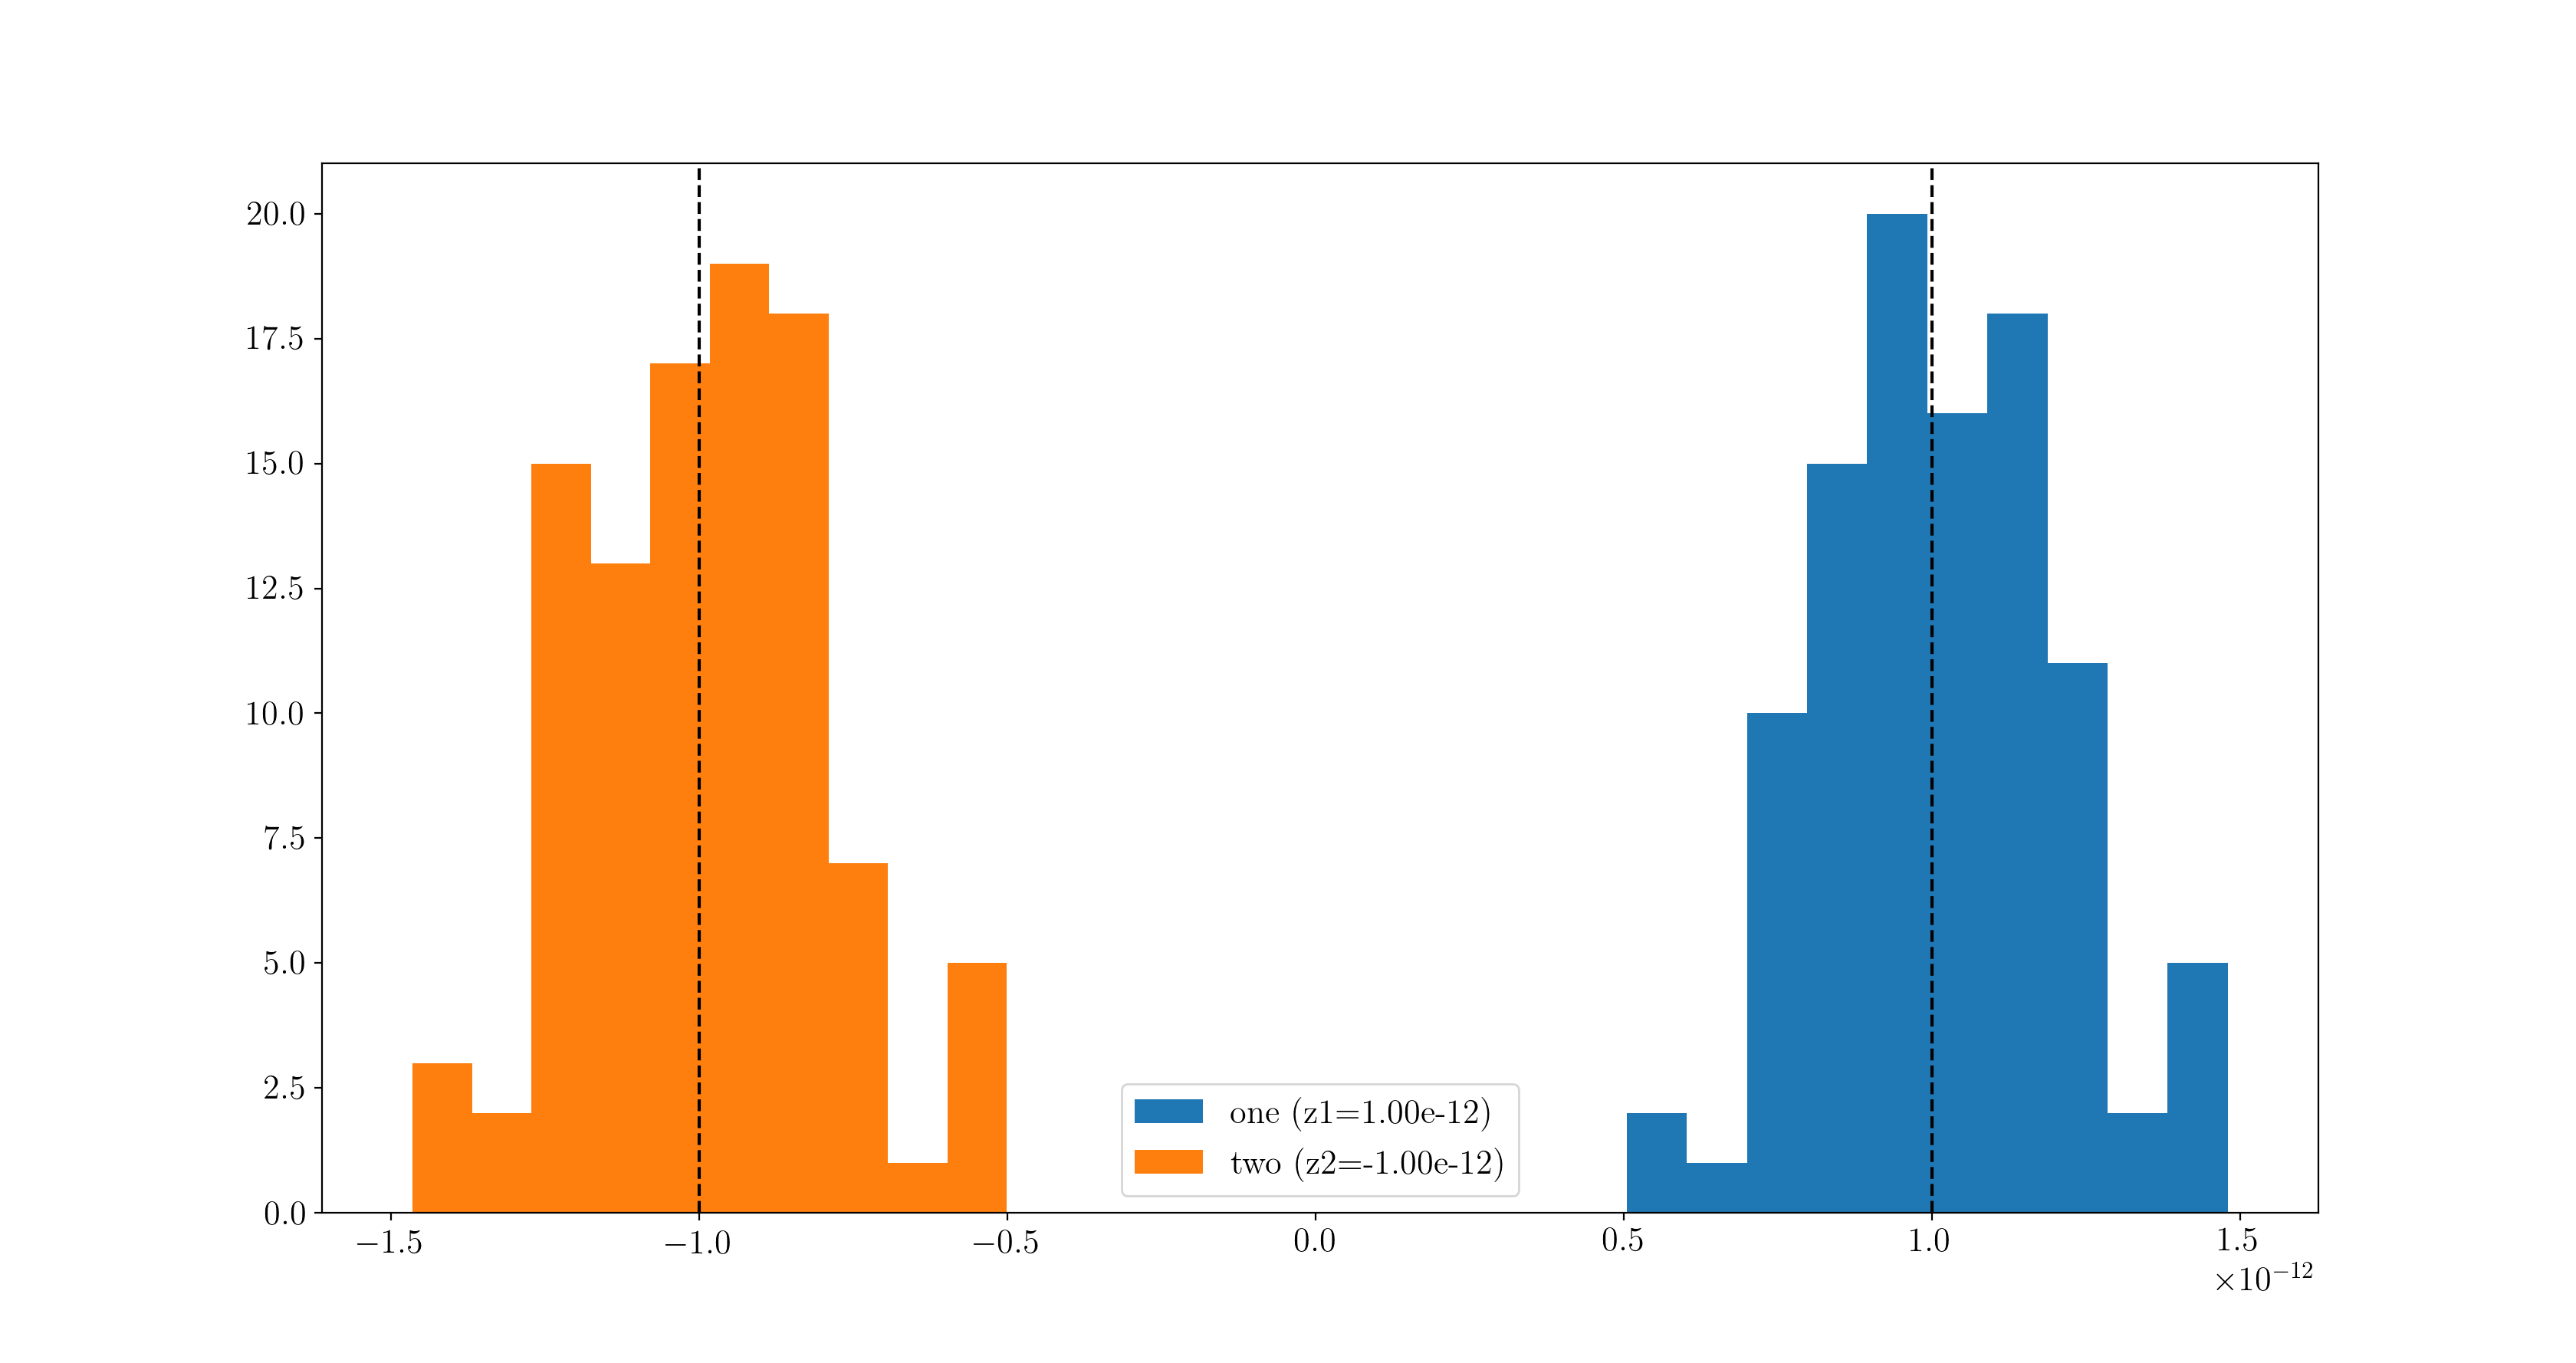
\includegraphics[width=\linewidth]{../../img/Koop/CO_offset_b1_b2_hist_vary_epsilons}
	\caption{Гистограммы распределений оценок $\hat{\Delta}^{\ntrl}$ в случае, когда варьируются только ошибки $\epsilon_1^{\ntrl},\epsilon_2^{\ntrl}$. \label{fig:vary_only_epsilons}}
\end{figure}

\begin{concl}
	$\sigma[\hat{\Delta}] = \sigSQUID/\sqrt{N_{BPM}\cdot N_{turn}}$.
\end{concl}

\section{Тест \# 2}
Добавляется вариация начальной фазы:
\[
	\phi_1^{\ntrl}, \phi_2^{\ntrl} \sim N\left(0, \pi\right).
\]

Результаты симуляции представлены на Рисунке~\ref{fig:vary_+phis}.

\begin{figure}[h]\centering
	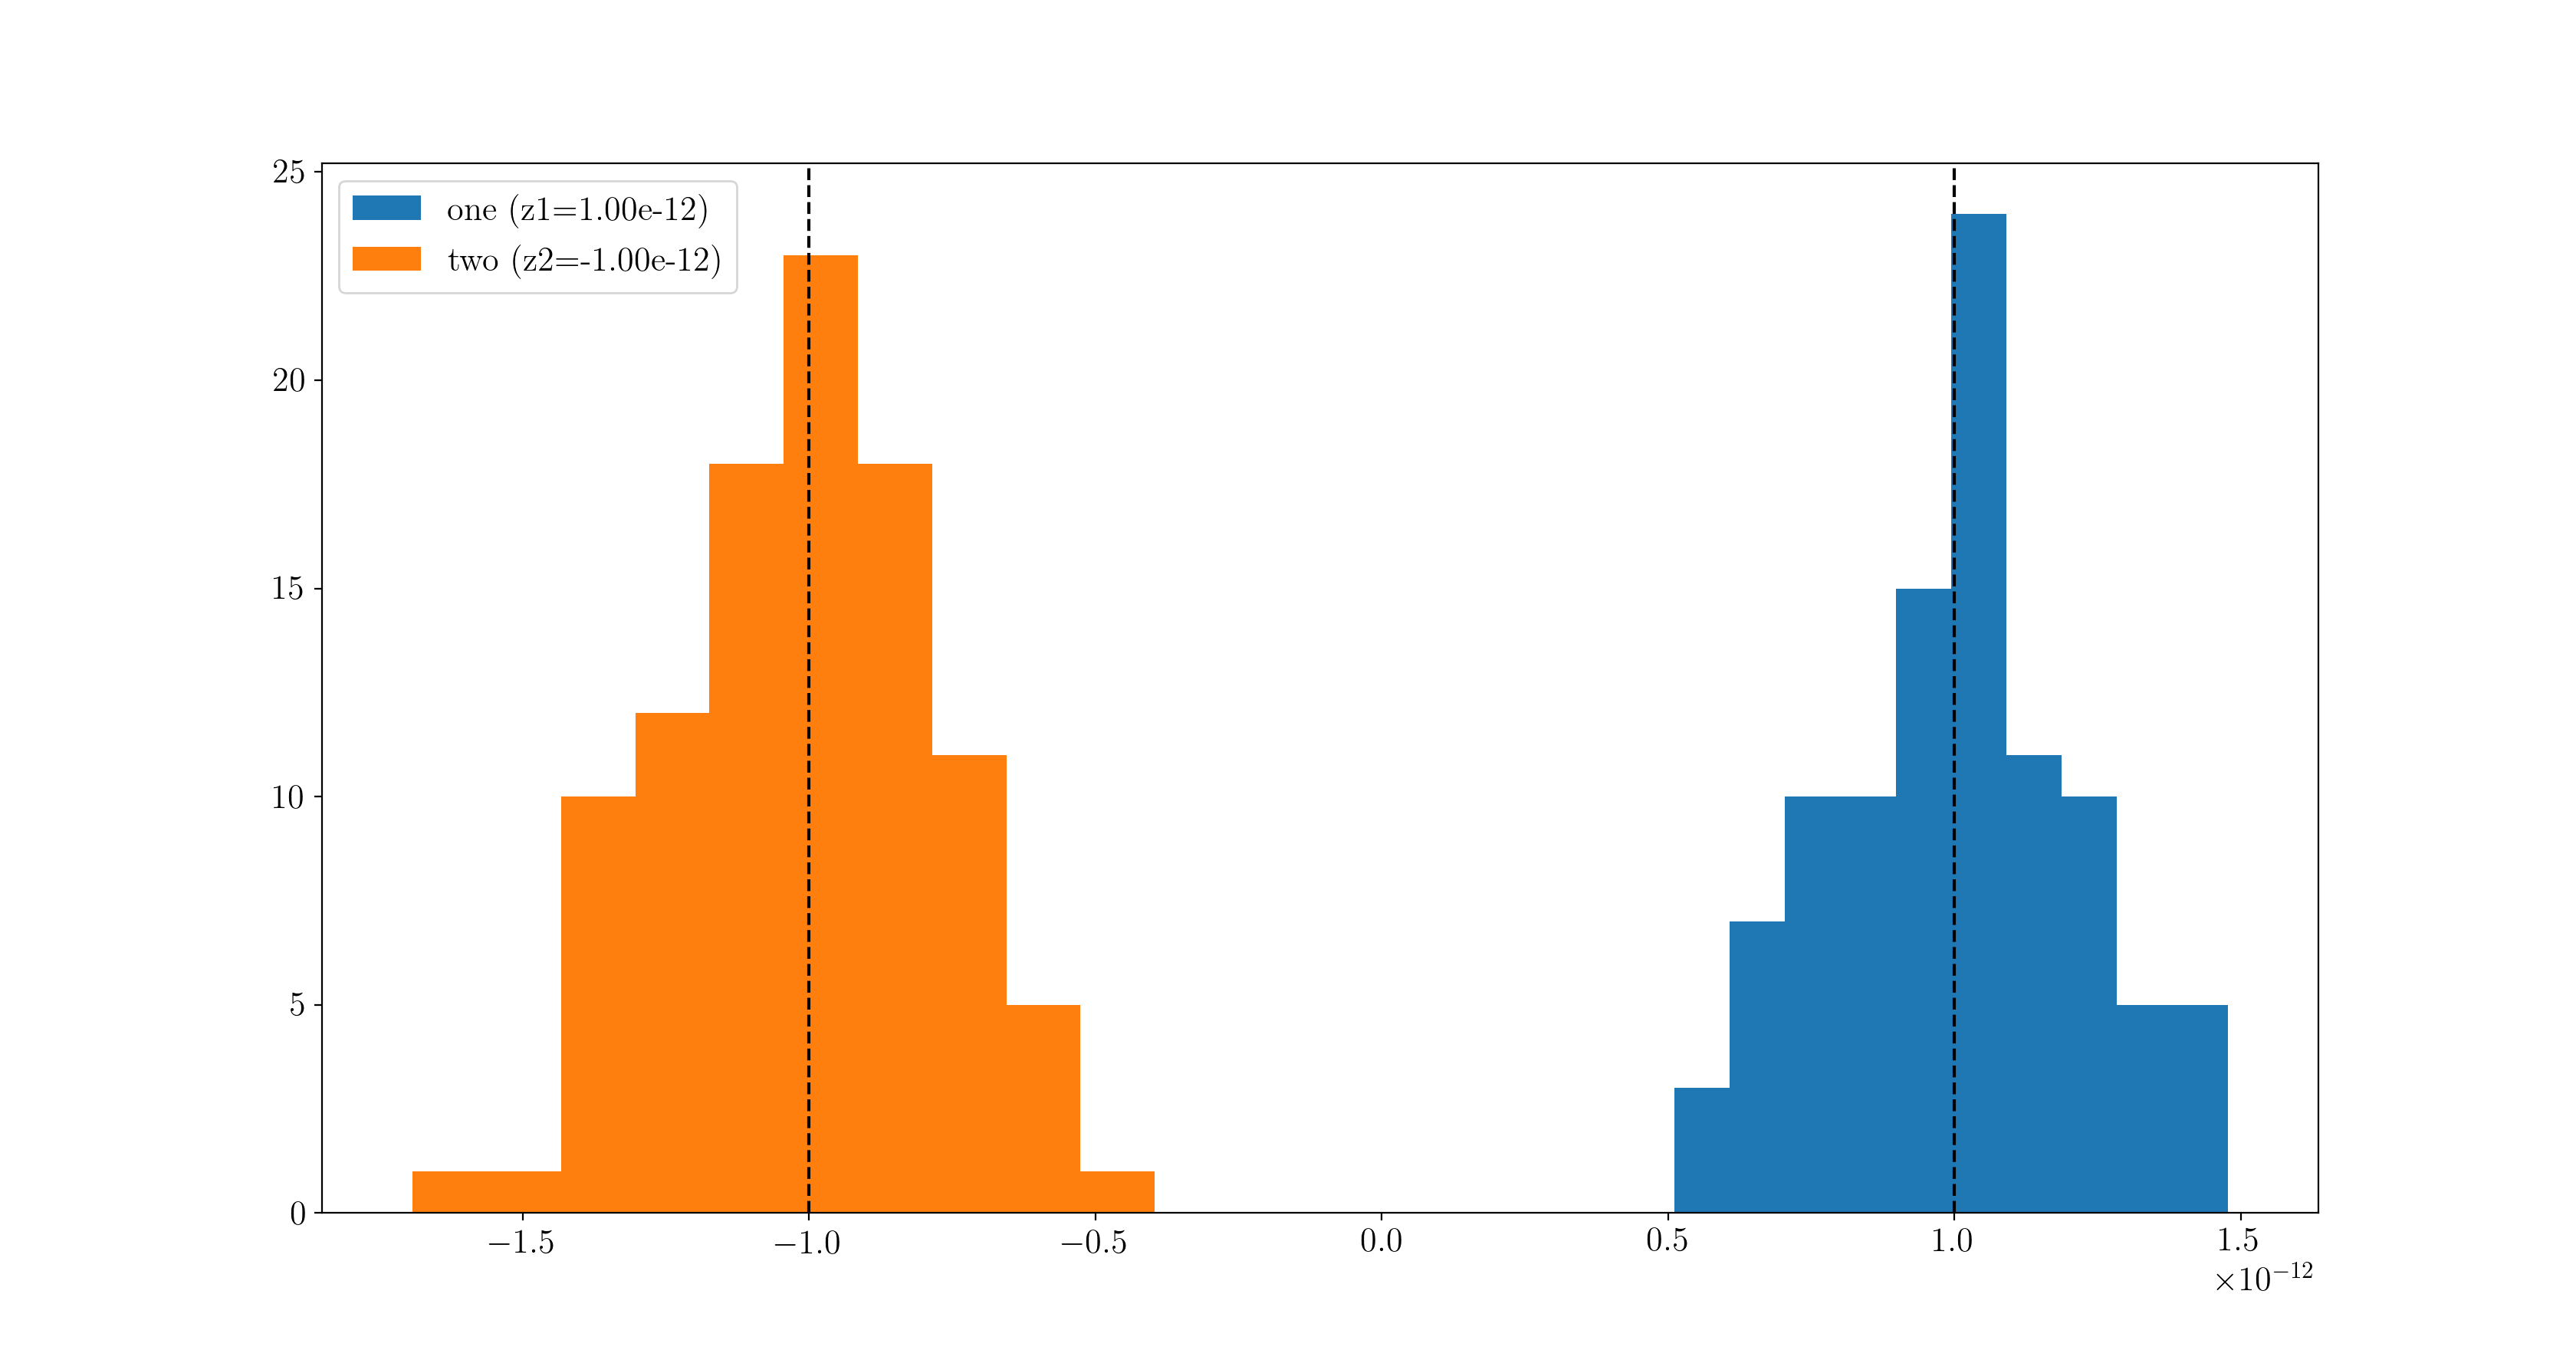
\includegraphics[width=\linewidth]{../../img/Koop/CO_offset_b1_b2_hist_vary_+phis}
	\caption{Гистограммы распределений оценок $\hat{\Delta}^{\ntrl}$ в случае, когда варьируются и ошибки $\epsilon_1^{\ntrl},\epsilon_2^{\ntrl}$, и начальные фазы $\phi_1^{\ntrl},\phi_2^{\ntrl}$ бетатронных колебаний. \label{fig:vary_+phis}}
\end{figure}

\begin{concl}
	Ничего не поменялось.
\end{concl}

\section{Тест \# 3}
Добавляем случайные отклонения частот:
\[
f_1^{\ntrl}, f_2^{\ntrl}\sim N(f_1, 10^{-3}),N(f_2,10^{-3}).
\]

\begin{rmk}
	Стандартные отклонения распределений частот не превышают $10^{-3}$ потому что иначе фиттер требует более близкие начальные оценки $\hat{f}$, а мне было лень писать умную функцию для этого.
\end{rmk}

Результаты симуляции представлены на Рисунке~\ref{fig:vary_+phis+freqs}.

\begin{figure}[h]\centering
	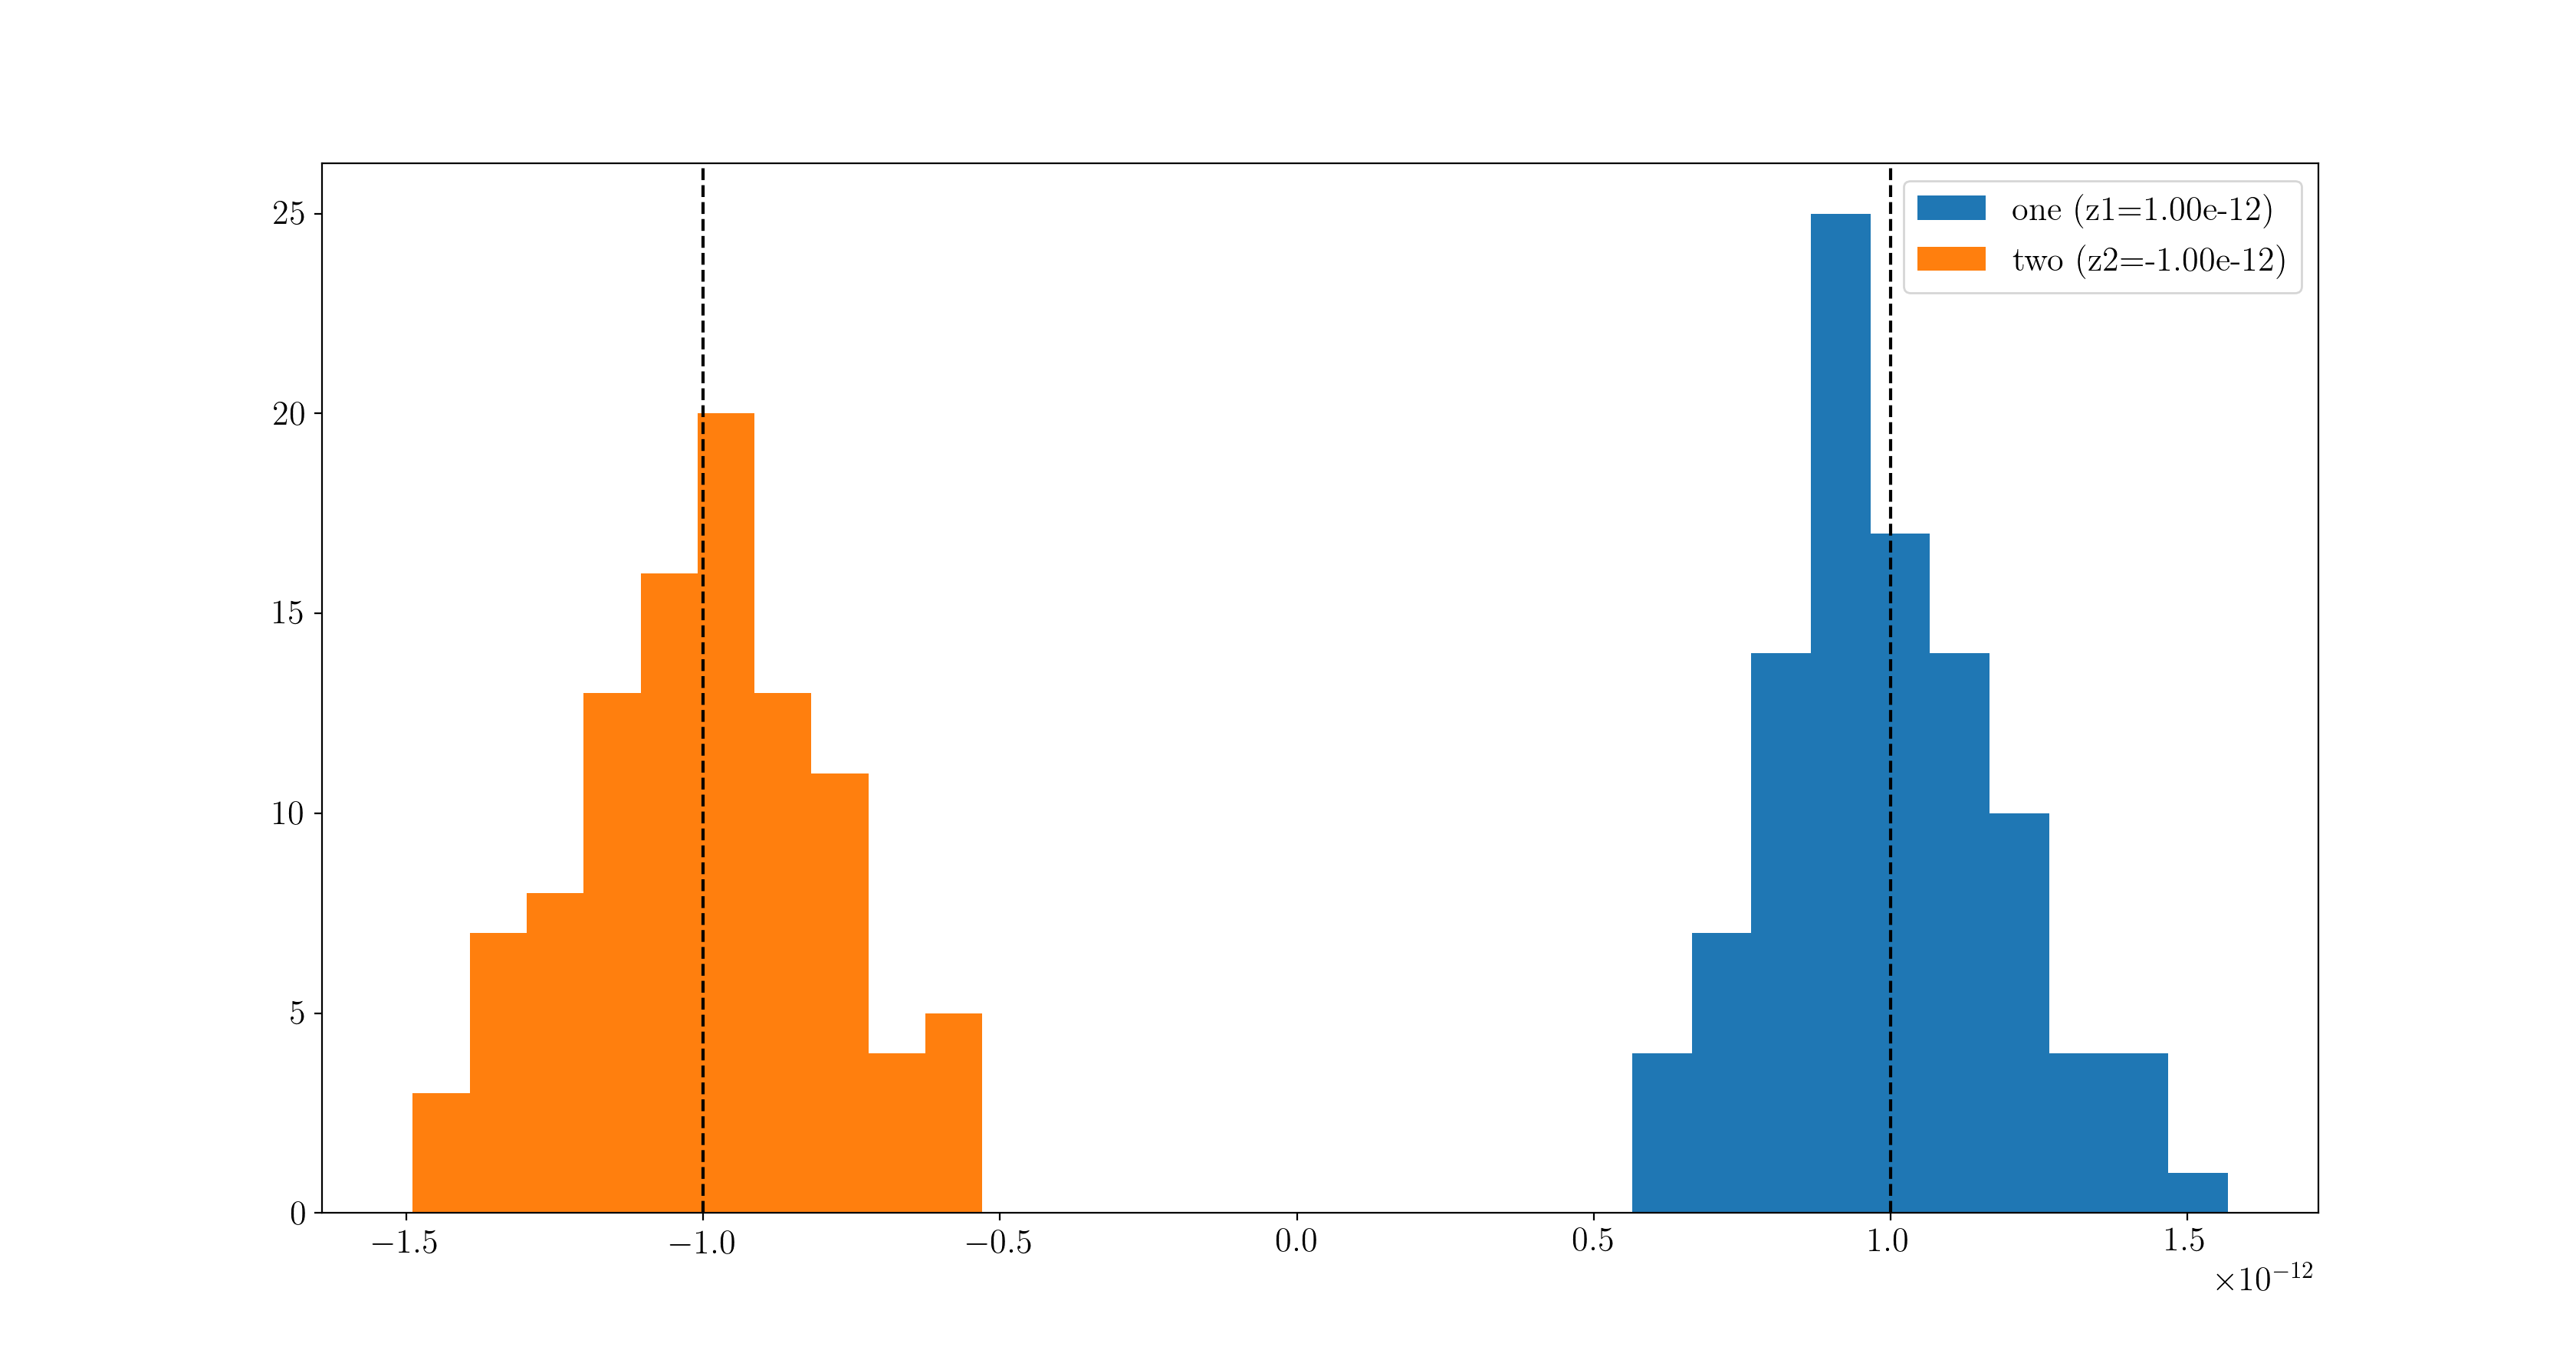
\includegraphics[width=\linewidth]{../../img/Koop/CO_offset_b1_b2_hist_vary_+phis+freqs}
	\caption{Гистограммы распределений оценок $\hat{\Delta}^{\ntrl}$ в случае, когда варьируются ошибки $\epsilon_1^{\ntrl},\epsilon_2^{\ntrl}$, начальные фазы $\phi_1^{\ntrl},\phi_2^{\ntrl}$, и частоты $f_1^{\ntrl},f_2^{\ntrl}$ бетатронных колебаний. \label{fig:vary_+phis+freqs}}
\end{figure}

\begin{concl}
	Снова никакой разницы.
\end{concl}

\section{Заключение}
По крайней мере, если мы можем определить остальные параметры вертикальных бетатронных колебаний (чтобы иметь возможность фитировать данные BPM'ов), мы должны быть в состоянии определить относительный вертикальный сдвиг замкнутых орбит пучков друг от друга с точностью локального измерения BPM.

Также, неправильно говорить, что если 

\end{document}